\documentclass[UTF8]{ctexart}

\usepackage[backend=bibtex]{biblatex}
\usepackage{mathtools}
\usepackage[CJKbookmarks=true,colorlinks,linkcolor=blue,anchorcolor=blue,citecolor=green]{hyperref}
\usepackage{color}
\usepackage{graphicx}
\usepackage{enumerate}
\usepackage{titlesec}
\usepackage{titletoc}
\usepackage{bm}

\newcommand{\HRule}{\rule{\linewidth}{0.5mm}}
\newcommand{\myFunc}{}
\newenvironment{myquote}
  {\begin{quote}\kaishu\zihao{-5}}
  {\end{quote}}

\titlecontents{section}
              [0em]
              {\bf \small}%
              {\contentslabel{2.5em}}%
              {}%
              {\titlerule*[0.5pc]{$\cdot$}\contentspage}%

\begin{document}
\begin{titlepage}
\begin{center}

\includegraphics[width=\textwidth]{UESTC-Logo}\\[2cm]
\textsc{\LARGE 计算机学院~$\bullet$~人工智能应用与挑战课程~}\\[1.5cm]
\HRule \\[0.4cm]
{ \huge \bfseries 血缘关系识别项目开题报告\\[0.4cm] }

\HRule \\[1.5cm]
\noindent
\emph{组名}:\quad
\quad {\bf Honkai StarRail}\\
\emph{作者}:\quad
\quad {\bf 刘*}\footnotemark
\quad {\bf 赵**}\footnotemark
\quad {\bf 武**}\footnotemark\\
\emph{指导老师}:\quad
\quad {\bf 文泉}
\end{center}
\footnotetext[1]{电子科技大学计算机科学与工程学院数字媒体技术专业,学号:2022**}
\footnotetext[2]{电子科技大学计算机科学与工程学院数字媒体技术专业,学号:2022**}
\footnotetext[3]{电子科技大学计算机科学与工程学院计算机科学与技术专业,学号:2022**}
\end{titlepage}

\tableofcontents
\newpage
\section{前言}
本篇报告为计算机学院~$\bullet$~人工智能应用与挑战课程~,Honkai StarRail小组的项目开题报告,小组选题为“Northeastern SMILE Lab - Recognizing Faces in the Wild”,(详见网址:\href{https://www.kaggle.com/competitions/recognizing-faces-in-the-wild}{小组选题})。

报告包括选题概况、题目分析、选题的最新研究状况、对选题所做的EDA、完成选题的基本思路与方法共五个部分,对所选题目进行初步分析。
\section{选题概况}
\subsection{选题内容}
本小组所选题目名为“Northeastern SMILE Lab - Recognizing Faces in the Wild”,中文直译为“东北大学微笑实验室-分辨野外的脸”,中文直译略有一些抽象,故本小组将其翻译为“基于图片实现血缘关系的鉴定”。

本题由东北大学的微笑实验室\footnote{Northeastern SMILE Lab}发起,其类型为Playground。

题目内容为:\footnote{引用自https://www.kaggle.com/competitions/recognizing-faces-in-the-wild}
\begin{quotation}
  In this competition, you’ll help researchers build a more complex model by determining if two people are blood-related based solely on images of their faces. If you think you can get it "on the nose," this competition is for you.
\end{quotation}

大意为训练一个图像识别模型,该模型能仅通过图像鉴定两人是否有血缘关系。由于用于亲属识别任务的现有图像数据库规模不足以捕捉和反映世界各地家庭的真实数据分布,并且许多隐藏因素会影响家族面部关系,因此需要比计算机视觉算法更有区分度的模型。

\subsection{选题意义}
当今社会,血缘关系鉴定有着多方面、多维度的社会意义:
\begin{itemize}
  \item 当家庭中存在怀疑亲子关系的情况时,血缘关系鉴定有助于维护家庭的稳定与和谐。
  \item 当在法律上出现亲子权纠纷、抚养权争议等问题时,血缘关系鉴定有利于保障当事人的合法权益。
  \item 当对某些人的身份存疑时,如失踪人员寻亲、被拐卖儿童寻亲等,血缘关系鉴定可帮助确认个人身份与亲属关系。
  \item 在医学上可以帮助研究家族遗传病的遗传模式、基因突变的传播等,辅助控制家族遗传病的产生。
\end{itemize}

而现如今最常用的血缘鉴定方式为依据遗传学的基本原理,采用现代化的DNA分型检测技术来综合评判争议个体之间是否存在亲生、隔代或其他血缘关系\footnote{详见https://baike.120ask.com/art/50356}。这种血缘关系鉴定需提取被鉴定者的DNA样本,并通过PCR扩增、后PCR反应、毛细管测序仪检测等步骤完成血缘鉴定,鉴定过程较为繁琐。若能开发出一套基于被鉴定者的外貌特征而实现的亲子鉴定系统,则将大大提高血缘鉴定的效率,减少血缘鉴定的成本。

\subsection{数据规模}

\begin{figure}[!ht]
  \centering
  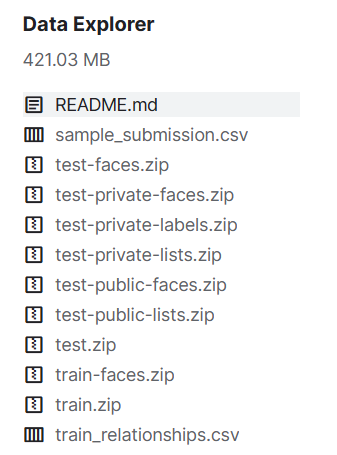
\includegraphics[width=0.5\textwidth]{training data.jpg}
  \caption{测试文件}
  \label{fig:training data}
\end{figure}

官方给出的测试数据共包含12个文件(详见图$\left(\ref{fig:training data}\right)$),其中较为重要的分别是:
\begin{itemize}
  \item train-faces.zip,训练集被分为家庭(F0123),然后是个体(MIDx)。同一MIDx文件夹中的图像属于同一个人。同一个F0123文件夹中的图像属于同一个家庭。
  \item train.csv,培训标签。其中需要注意的是,一个家庭中并不是每个成员都有亲属关系。例如,父母与他们的孩子有亲属关系,但彼此之间没有亲属关系。
  \item test-faces.zip,该测试集中包含未知个体的人脸图像。
  \item sample\underline{\space}submission.csv,该文件为一个正确格式的示例提交文件。列\\
  img\underline{\space}pair描述了图像对,即abcd-efgh表示图像对abcd.jpg和efgh.jpg。\\
  我们的目标是预测test-faces中每对图像是否相关,其中1表示相关,0表示不相关。
\end{itemize}

以上数据文件总大小为421.03MB。

\subsection{比赛现状}

\begin{figure}[!ht]
  \centering
  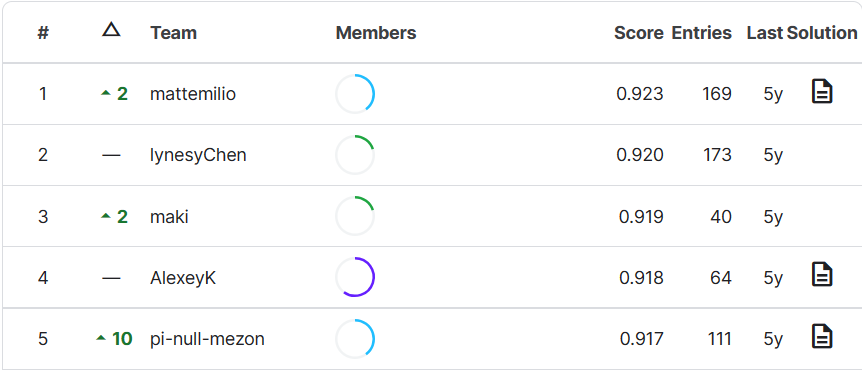
\includegraphics[width=0.7\textwidth]{leaderboard.jpg}
  \caption{排行榜1-5名}
  \label{fig:leaderboard}
\end{figure}

截至目前,共有573位参赛选手,522支参赛队伍。由于该题在五年前已完赛,故参赛选手的最终提交时间均在五年之前。

在该题目的leaderboard中(见图$\left(\ref{fig:leaderboard}\right)$),目前的世界第一为mattemilio,其得分为0.923分,前五名得分均在0.917之上。

\section{题目分析}
为了进一步了解该选题模型的特点并推进小组工作,我们需对该选题进行定性的分析。
\subsection{PEAS}

我们通常用PEAS 去描述一个任务所处的环境,其中P 指性能指标($\textit{Performance measure}$)、E 指外部环境($\textit{External environment}$)、A 指执行器($\textit{Actuators}$)、S 指传感器($\textit{Sensors}$),现在我们同样用PEAS 对本次竞赛的任务进行描述:

\begin{itemize}
  \item \textbf{Performance measure}:该题的性能度量主要由识别血缘关系的正确率来衡量,除此之外,我们也认为血缘关系识别的效率也影响该模型的性能。
  \item \textbf{External environment}:该题的外部环境涉及被识别人像的姿势、面部表情、环境光照、图像背景、图像噪声、图像的分辨率等。
  \item \textbf{Actuators}:该题的执行器主要有对数据的预处理,使图像易于我们的模型采样与识别,同时也包括图像处理算法与血缘关系判别算法。
  \item \textbf{Sensors}:我们小组采用人脸图像白化处理矩阵来采集图中的人脸信息,故传感器为人脸图像白化处理矩阵。
\end{itemize}

\subsection{七维分类}
仔细阅读题目后,我们小组采用七个维度对该题进行了分类:

\begin{enumerate}
  \item \textbf{Fully observable},用于识别是否具有血缘关系的两张人像图片均可以观测,模型始终能够完全且准确地获知被识别的人脸信息。
  \item \textbf{Single agent},所训练的模型为单一智能体,只需考虑自身决策,判断输入的两张图片中的人是否具有血缘关系。
  \item \textbf{Stochastic},面部图像识别的过程本质上受到光线、表情、图像噪声等环境因素影响,此不确定的环境因素可能会导致识别结果的不确定性,因此属于随机环境。
  \item \textbf{Episodic},每次进行血缘关系识别的任务都是相互独立的,模型做出的决策不会受到之前识别结果的影响,因此属于Episodic。
  \item \textbf{Static},用于识别是否具有血缘关系的两张人像图片均是静止的,不会发展或产生外界变化。
  \item \textbf{Discrete},模型在识别时采样的特征有限,因而采样的数据点有限,且数据点之间互为离散关系。
  \item \textbf{Known},模型完全能掌握与了解输入图像的特性,以判断两张图像中的人物是否具有血缘关系。
\end{enumerate}

\section{最新研究现状}
在基于图片实现血缘关系鉴定的研究中,我们小组从网上了解到最新的研究包括GenoFace\footnote{结合基因组学信息和人脸图像数据的血缘关系识别项目。}、FamiliFace\footnote{基于家族数据集的人脸识别项目,旨在识别家族成员之间的血缘关系。}、LineageLens\footnote{通过深度学习技术探索人脸图像中的遗传线索,以识别血缘关系的项目。}、ProgenyProbe\footnote{利用人工智能技术研究人脸图像中的遗传特征,从而确定人物之间的亲属关系。}、KinshipConnect\footnote{通过分析人脸图像数据来建立亲属关系网络的项目。}、HeritageMatcher\footnote{利用深度学习算法匹配人脸图像中的遗传特征,以确定人物之间的血缘关系。}、PedigreePix\footnote{通过人脸识别技术建立家族谱系的项目,用于确定人物之间的亲属关系。}等,本篇开题报告中仅介绍KinshipConnect与GenoFace。

\begin{figure}[!ht]
  \centering
  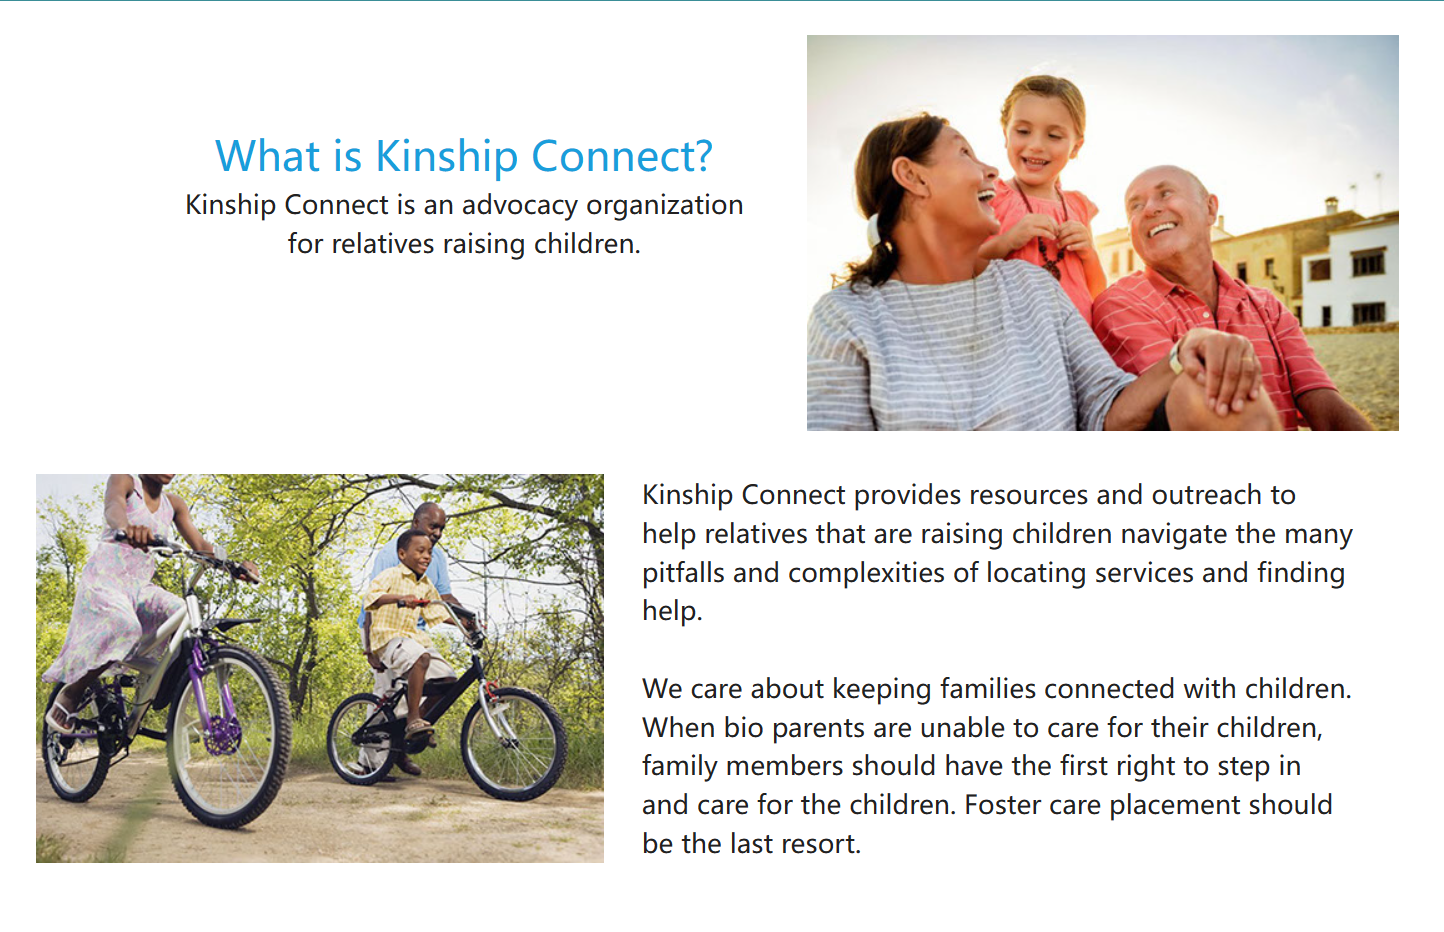
\includegraphics[width=0.8\textwidth]{KinshipConnect.png}
  \caption{KinshipConnect}
  \label{fig:KinshipConnect}
\end{figure}

\subsection{KinshipConnect}
KinshipConnect\footnote{http://kinshipconnect.org/}是一个非盈利性组织,该平台旨在帮助家庭成员之间更轻松地保持联系和分享信息,通过上传家族成员图片,用户可以轻松地构建和管理他们的家庭树。用户可以上传家族历史文档、照片和视频,以及记录家族传统和故事,从而帮助保存家族的文化遗产(见图$\left(\ref{fig:KinshipConnect}\right)$)。

\subsection{GenoFace}
Genoface项目采用卷积神经网络(CNN)和生成对抗网络(GAN),对图片集进行训练。通过分析个体的基因组数据,预测其外貌特征,包括但不限于肤色、眼睛颜色、发色等判断不同人之间的基因关系。期望将训练结果运用于犯罪学、人类演化学、医学遗传学等领域(见图$\left(\ref{fig:GenoFace}\right)$)。

\begin{figure}[!ht]
  \centering
  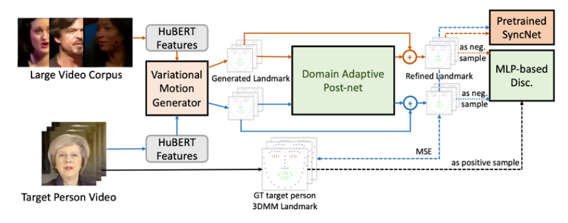
\includegraphics[width=0.8\textwidth]{GenoFace.png}
  \caption{GenoFace}
  \label{fig:GenoFace}
\end{figure}

\section{进行EDA}
\subsection{关于EDA}
\subsubsection{定义}
探索性数据分析(Exploratory Data Analysis,简称EDA)是一种统计学和数据分析方法,其目的是通过可视化、摘要统计和图形化方法来分析数据集,以便发现数据的模式、趋势、异常值和联性等。EDA 的主要目标是在深入了解数据之前,为进一步分析或建模做准备。
\subsubsection{主要步骤}
EDA通常包括以下步骤:
\begin{enumerate}
  \item \textbf{数据可视化}:通过绘制图表、图形等方式将数据可视化,帮助我们直观地了解数据的分布、关系等。
  \item \textbf{数据概要统计}:计算数据的一些基本统计量,如均值、中位数、方差等,以了解数据的中心趋势和离散程度。
  \item \textbf{数据清洗}:检查和处理数据中的缺失值、异常值等问题,确保数据的质量和可靠性。
  \item \textbf{特征工程}:对数据进行特征提取、选择和转换,以便更好地适应后续的分析方法。
  \item \textbf{数据分析和模型选择}:根据数据的特点和分析目的,选择合适的分析方法和模型进行进一步的分析。
\end{enumerate}
\subsubsection{优点}
EDA的优点在于它可以帮助我们小组快速了解选题所给数据的基本特征和规律,发现数据中的潜在问题和异常情况,为后续的深入分析和建模提供有益的信息和启示。同时,EDA 也可以帮助我们更好地理解数据,激发数据分析的灵感,提出更有针对性的问题和假设。

\subsection{本题EDA}%
将数据从kaggle网页上下载之后,我们小组对其进行了EDA操作。
\begin{enumerate}
  \item 首先找到所有的训练图像,并将它们存储到一个数据结构中。为了准备训练图像的文件路径,以便后续的数据处理和模型训练。(详细:遍历文件夹,找到所有的训练图像,并将它们的路径储到一个列表 train\_li 中。然后,代码创建一个包含所有训练图像路径的字典
  train\_file\_dict,这个字典将图像路径映射到它们的索引位置。最后,代码创建了一个名为 train\_file\_df 的 Pandas DataFrame,用于存储训练图像的文件路径。)下图$\left(\ref{fig:EDA1}\right)$为其中的一些样本路径:
  \begin{figure}[!ht]
    \centering
    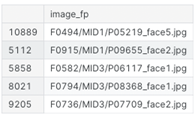
\includegraphics[width=0.3\textwidth]{EDA1.png}
    \caption{样本路径}
    \label{fig:EDA1}
  \end{figure}
  \item 寻找具有亲属关系的图像对,对训练集中的每一对亲属关系进行处理,并提取出有亲属关系的图像对,将它们存储在一个名为 
  train\_pairs\_kinship 的DataFrame中,图$\left(\ref{fig:EDA2}\right)$展示了其中的一些样本,包含列 p1 和 p2,分别代表图像对中的第一个和第二个图像的索引。
  \begin{figure}[!ht]
    \centering
    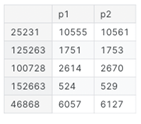
\includegraphics[width=0.3\textwidth]{EDA2.png}
    \caption{具有血缘关系的图像索引}
    \label{fig:EDA2}
  \end{figure}
  \item 因为我们正在训练一个模型来识别两张图像的相似性,而同一个人被认为具有血缘关系。创建属于同一个人的图像对,图$\left(\ref{fig:EDA3}\right)$为其中同一人的样本索引值:
  \begin{figure}[!ht]
    \centering
    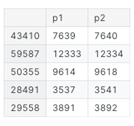
\includegraphics[width=0.3\textwidth]{EDA3.png}
    \caption{同一人的图像索引}
    \label{fig:EDA3}
  \end{figure}
  \item 图$\left(\ref{fig:EDA4}\right)$展示了官方所给训练文件中的具有亲属关系的图像对和来自同一个人的图像对的数量对比。
  \begin{figure}[!ht]
    \centering
    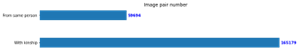
\includegraphics[width=0.7\textwidth]{EDA4.png}
    \caption{具有亲缘关系与同一人的图像数量对比}
    \label{fig:EDA4}
  \end{figure}
  \item 将具有亲属关系的图像对和来自同一个人的图像对合并到一起,合并后的具有亲属关系的图像对的总数为224873。
  \item 获取数据集中所有可能的图像对,无论这些图像是否属于同一个人或具有亲属关系。
  \item 根据图像对是否具有亲属关系,为数据集中的图像对增加了一个名为 "is\_related" 的特征列,如果图像对具有亲属关系则标记为1,否则标记为0。
  \item 显示具有亲属关系和不具有亲属关系的图像对数量对比,详见图$\left(\ref{fig:EDA5}\right)$。
  \begin{figure}[!ht]
    \centering
    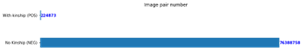
\includegraphics[width=0.7\textwidth]{EDA5.png}
    \caption{具有亲缘关系与不具有亲缘关系的数量对比}
    \label{fig:EDA5}
  \end{figure}
  \item 为每个图像获取家庭ID。从图像文件路径中提取家庭ID,并将其存储在数据框的新列中。图$\left(\ref{fig:EDA6}\right)$展示了添加家庭ID后的数据结果。打印发现训练集中家庭的数量为470。
  \begin{figure}[!ht]
    \centering
    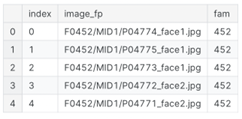
\includegraphics[width=0.3\textwidth]{EDA6.png}
    \caption{添加家庭ID后的数据样例}
    \label{fig:EDA6}
  \end{figure}
  \item 为每对具有亲属关系的图像中的第一个图像添加家庭ID,添加后的结果如图$\left(\ref{fig:EDA7}\right)$所示。
  \begin{figure}[!ht]
    \centering
    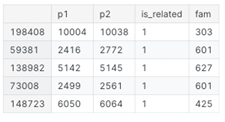
\includegraphics[width=0.3\textwidth]{EDA7.png}
    \caption{添加家庭ID后的数据样例}
    \label{fig:EDA7}
  \end{figure}
  \item 图$\left(\ref{fig:EDA8}\right)$展示了具有亲属关系的图像对中前20个家庭的样本数量分布。
  \begin{figure}[!ht]
    \centering
    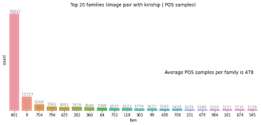
\includegraphics[width=0.6\textwidth]{EDA8.png}
    \caption{前20个家庭的样本数量分布}
    \label{fig:EDA8}
  \end{figure}

  可以发现样本分布存在严重问题,打开家庭文件夹后,会发现它是英国王室。所以需要限制每个家庭的样本数,设定样本数上限为3000,然后找到超过这一限制的家族。对于超过限制的家族,我们随机抽取3000个样本。调整之后如图$\left(\ref{fig:EDA9}\right)$所示。
  \begin{figure}[!ht]
    \centering
    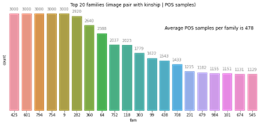
\includegraphics[width=0.6\textwidth]{EDA9.png}
    \caption{调整后的样本数量分布}
    \label{fig:EDA9}
  \end{figure}
  \item 接下来,我们定义了几个图像预处理函数:
  \begin{verbatim}
    def prewhiten(x):
      if x.ndim == 4:
          axis = (1, 2, 3)
          size = x[0].size
      elif x.ndim == 3:
          axis = (0, 1, 2)
          size = x.size
      else:
          raise ValueError('Dimension should be 3 or 4')
  
      mean = np.mean(x, axis=axis, keepdims=True)
      std = np.std(x, axis=axis, keepdims=True)
      std_adj = np.maximum(std, 1.0/np.sqrt(size))
      y = (x - mean) / std_adj
      return y

    def l2_normalize(x, axis=-1, epsilon=1e-10):
      output = x / np.sqrt(np.maximum(np.sum(np.square(x), 
      axis=axis, keepdims=True), epsilon))
      return output
  \end{verbatim}
  其中prewhiten函数的作用是对输入的图像进行白化处理,使得图像数据的分布具有零均值和单位方差。这样做可以降低特征之间的相关性,有助于提高模型训练的收敛速度和性能。l2\_normalize函数用于对输入的向量进行L2范数归一化,即将向量的每个元素除以其L2范数,从而将向量映射到单位范数的空间中。
  
\end{enumerate}

\section{解题基本思路、方法与技术路线}
\subsection{解题思路}
题目中给出了特定的训练集、验证集、测试集三类文件,要求依据训练图片集训练模型,由验证图片集计算训练效果,最终上传至kaggle,由kaggle中的测试集测试模型拟合程度,依据模型判断的成功率计算得分。\\
所以我们的思路集中在首先提取面部特征,对数据处理后,传入现有的图片对比模型进行训练,然后测试验证图片集,得到模型测试准确度,进一步在根据验证集训练模型,最后将训练合适次数的模型传入kaggle。

\subsection{解题方法}
解题方法大致分为两个步骤:
\begin{enumerate}
  \item \textbf{提取图片特征}:通过比对VGGface、FaceNet、DeepFace的优缺点后,我们选用适合当下数据规模的FaceNet模型(图$\left(\ref{fig:FaceNet}\right)$)进行图片特征的提取。
  
  \begin{figure}[!ht]
    \centering
    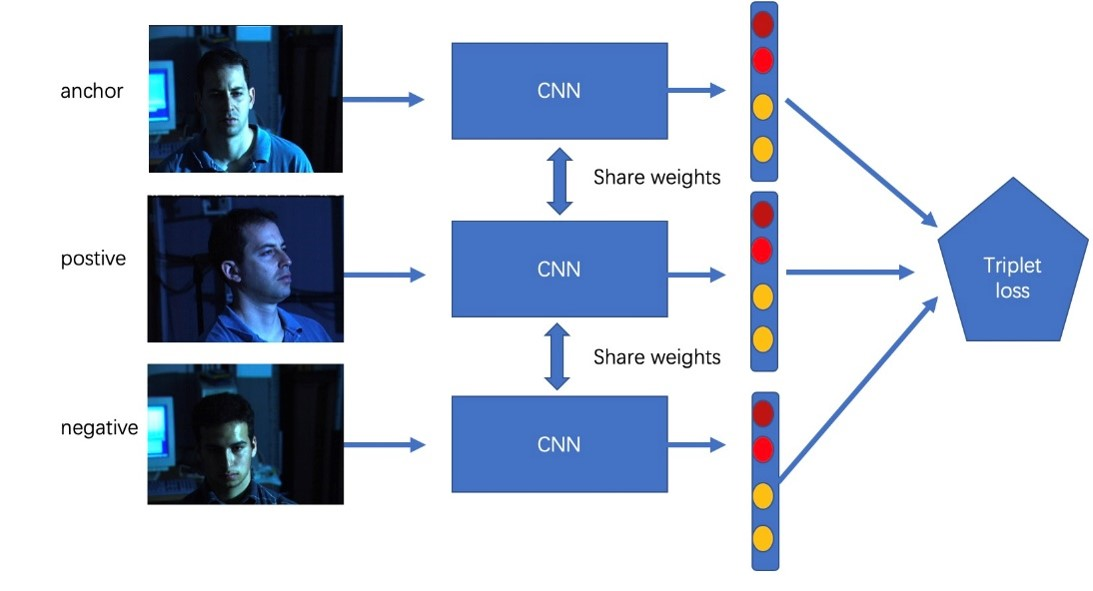
\includegraphics[width=0.8\textwidth]{FaceNet.jpg}
    \caption{FaceNet}
    \label{fig:FaceNet}
  \end{figure}

  \item \textbf{训练图片处理模型}:由于本问题虽然是图片比对问题,但其实并不算是一个分类问题,即该问题并不需要给每个图片划分标签。问题只需要的是判断两张图片的相似性。由此我们选用了不带标签的孪生神经网络(Siamese Network)解决该问题。在Siamese Network中,将两张图片的特征值抽象为两个向量值X1,X2,通过公式\[L(W,(Y,X_1,X_2))=\frac{1}{2N}\sum_{n=1}^{N}YD^2_W+(1-Y)max(m-D_W,0)^2\],其中\[D_W(X_1,X_2)=||X_1-X_2||_2=(\sum_{i=1}^{P}(X^i_1-X^i_2)^2)^\frac{1}{2}\]得到loss函数,进而判断X1向量与X2向量的相似程度。
\end{enumerate}

前期的思路除了确定模型采用之外,我们的目光主要聚焦于数据预处理上。


对于图片预处理,我们使用了以下几种技术:
\begin{enumerate}
  \item \textbf{白化处理}:由于图片集中,每张图片的色彩分布均有不同的不均衡,故我们采用白化处理使图片像素分布更均衡。具体方法为:先计算图像像素均值和方差,其中均值计算公式为:\[\mu =\frac{\sum_{i=1}^{I}\sum_{j=1}^{J}p_{ij}}{IJ}\]方差计算公式为:\[\sigma^2 = \frac{\sum_{i=1}^{I}\sum_{j=1}^{J}(p_{ij}-\mu)^2}{IJ}\]白化处理后的像素点值为:\[x_{ij}=\frac{p_{ij}-\mu}{\sigma}\]
  \item \textbf{图像颜色通道对齐处理}:对颜色通道有偏差的图片,使用矩阵\[
    \begin{bmatrix}
      x_1\\y_1\\1\\
    \end{bmatrix}=H
    \begin{bmatrix}
      x_2\\y_2\\1\\
    \end{bmatrix}=
    \begin{bmatrix}
      h_{00}&h_{01}&h_{02}\\
      h_{10}&h_{11}&h_{12}\\
      h_{20}&h_{21}&h_{22}\\
    \end{bmatrix}
    \begin{bmatrix}
      x_2\\y_2\\1\\
    \end{bmatrix}\]对齐RGB通道。对齐结果如图$\left(\ref{fig:ECC}\right)$所示。
    \begin{figure}[!ht]
      \centering
      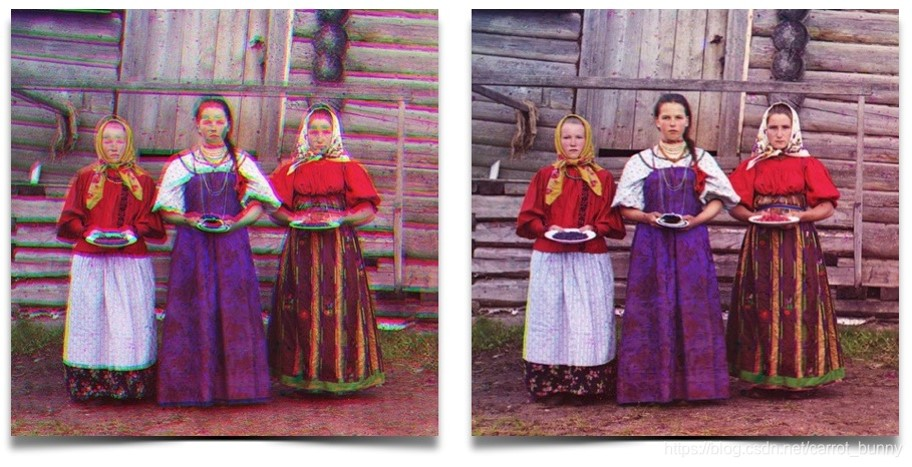
\includegraphics[width=0.7\textwidth]{ECC.jpg}
      \caption{RGB通道对齐样例}
      \label{fig:ECC}
    \end{figure}
  \item \textbf{归一化}:对输入向量进行L2范数归一化,增强图像鲁棒性和可比性。
  \item \textbf{面部对齐}:使用Yolov5算法进行目标检测,识别脸部位置。
  \item \textbf{Homography法}:利用特征对齐图像,将旋转的图像重新对齐,以便于我们对模型的训练。
\end{enumerate}

\section{参考文献}

\begin{thebibliography}{99}
  \bibitem{1} Koch, G., Zemel, R., \& Salakhutdinov, R. (2015). Siamese Neural Networks for One-shot Image Recognition. In Proceedings of the 32nd International Conference on Machine Learning (ICML) (Vol. 37, pp. 1774-1782).
  \bibitem{2} Taigman, Y., Yang, M., Ranzato, M., \& Wolf, L. (2014). DeepFace: Closing the Gap to Human-Level Performance in Face Verification. In Proceedings of the IEEE Conference on Computer Vision and Pattern Recognition (CVPR) (pp. 1701-1708).
  \bibitem{3} Chopra, S., Hadsell, R., \& LeCun, Y. (2006). A Probabilistic Framework for Semi-Supervised Clustering. In Proceedings of the 10th European Conference on Computer Vision (ECCV) (pp. 161-174). Springer Berlin Heidelberg.
  \bibitem{4} Bromley, J., Guyon, I., LeCun, Y., Sackinger, E., \& Shah, R. (1994). Signature Verification using a "Siamese" Time Delay Neural Network. In Advances in Neural Information Processing Systems 6 (NIPS) (pp. 737-744).
  \bibitem{5} Hadsell, R., Chopra, S., \& LeCun, Y. (2006). Dimensionality Reduction by Learning an Invariant Mapping. In Proceedings of the IEEE Conference on Computer Vision and Pattern Recognition (CVPR) (Vol. 2, pp. 1735-1742).
  \bibitem{6} Lawrence, S., Giles, C. L., \& Tsoi, A. C. (1997). Face Recognition: A Convolutional Neural Network Approach. In Advances in Neural Information Processing Systems 10 (NIPS) (pp. 766-772).
\end{thebibliography}

\end{document}
